% !Mode:: "TeX:UTF-8"
\documentclass[11pt]{article}
\usepackage[letterpaper, margin = 2cm]{geometry}
\usepackage{microtype}
\usepackage{parskip}
\usepackage{amssymb}
\usepackage{amsmath}
\usepackage{multicol}
\usepackage{graphicx}
\usepackage{caption}
\usepackage[style=ieee]{biblatex}
\usepackage[bookmarks, unicode]{hyperref}

\addbibresource{references.bib}

\title{Heat Flux}
\author{Josh Kraan}
\date{\today}

\begin{document}

\maketitle

\section{Gas Properties}

Combustion gas properties are commonly calculated using NASA's Chemical Equilibrium with Applications (CEA) \cite{} program, however this FORTRAN program is difficult to integrate with. Instead the combustion gas properties are calculated using Cantera as described by Youngblood \cite{}. Species included in the chemical equilibrium calculations are based off of those used in CEA and kerosene combustion models \cite{} as well as the availability of tranport properties. The species included in this analysis are: RP-1, LOX, CO, CO2, H, H2, H2O, O, OH, and O2. RP-1 and LOX are modelled with the same stoichiometry and heat of formation as used in CEA. Cantera requires transport properties for all species, so RP-1 and LOX are assigned placeholder values with the understanding that equilibirum solutions will contain essentially zero concentration of these species. Thermodynamic properties are taken from NASA \cite{}, and Lennard-Jones transport properties are taken from the GRI MECH 3.0 combustion mechanism \cite{}.

%TODO gri transport property valid range

\subsection{Axial Variation}


Chamber properties are calculated using the same method as Youngblood, and two nested root finders are used to calculate gas properties throughout the converging-diverging sections of the engine. The outer root finder solves the isentropic flow relation for pressure: %TODO cite

\begin{equation}
  \frac{p}{p_0} = (1 + \frac{\gamma - 1}{2} M^2) ^ {- \frac{\gamma}{\gamma - 1}}
\end{equation}

The specific heat ratio for the combustion gas is calculated at each evaluated pressure and the chamber entropy. The specifc heat ratio and the area ratio are used to solve the mach number equation using the other root finder. Subsonic or supersonic solutions are forced by changing the bracketing interval depending on axial location.

\begin{equation}
    \left( \frac{A}{A_t}\right)^2 = \frac{1}{M^2} \left\{ \frac{2}{\gamma + 1} \left[ 1 + \frac{1}{2} (\gamma - 1) M^2 \right] \right\}^{\frac{\gamma + 1}{\gamma - 1}}
\end{equation}

\subsection{Frozen Boundary Layer Chemistry}

CEA calculates ``frozen'' and ``equilibrium'' values for specific heat and thermal conductivity. Equilibrium values are taken to be the sum of the frozen value and a reaction term that accounts for chemical reactions occuring in the boundary layer. Equilibirum values for both are several times higher than frozen, and using the equilibrium values would lead to a calculated heat flux approximately 4.5 times higher (based on the Bartz equation).

Bartz \cite{page 46} discusses chemical reactions occuring in rocket engine boundary layers and the resulting increase in heat transfer. When dissociated species such as O, H, and OH are present in the free stream, they can cool against combustion walls and recombine exothermically in the boundary layer. Bartz notes that this effect would likely be maximum for a hydrogen and oxygen rocket at 100\% combustion efficiency, yet the increase in heat flux over a frozen layer is shown to be only 32\% and rapidly decreases with reduced combustion efficiency.

The presence of dissociated species is not insigificant for this engine, as can be seen in figure \ref{}. It is unclear why equilibirum values calculated by CEA are so high and reproducing them is difficult, so based off of the Bartz information the boundary layer will be considered to be chemically frozen.


\begin{minipage}{.5\linewidth}
  \centering
  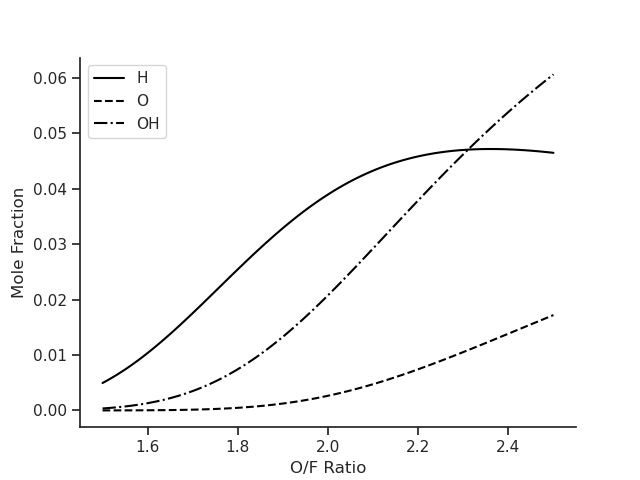
\includegraphics[width=\linewidth]{dissociated-chamber.png}
  \captionof{figure}{Chamber dissociated species.}
\end{minipage}%
\begin{minipage}{.5\linewidth}
  \centering
  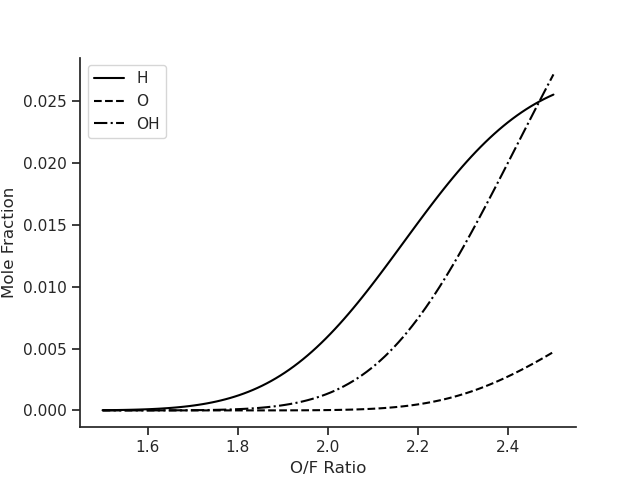
\includegraphics[width=\linewidth]{dissociated-nozzle.png}
  \captionof{figure}{Nozzle dissociated species.}
\end{minipage}

%TODO species for OF ratio graph to support this

\subsection{Frozen Contraction and Expansion}

Through the contraction and expansion of the engine, combustion gas can be considered to either be in equilibrium (mole fractions change along length of engine) or the composition could be frozen. Both methods are implemented, but this was found to make little difference to heat flux calculations.

%TODO look into more

\subsection{Property Comparison}

\section{Heat Flux Models}

\subsection{Bartz}

The Bartz equation is commonly used for calculating rocket engine heat flux. The following form is common:

\begin{equation}
    \label{equation:bartz}
    \begin{split}
         h_g = \left[ \frac{0.026}{D_t^{0.2}} \left( \frac{\mu^{0.2} C_p}{{Pr}^{0.6}} \right)_{ns} \left( \frac{(p_c)_{ns}}{c^*} \right)^{0.8} \left( \frac{D_t}{R_c} \right)^{0.1} \right] \left( \frac{A_t}{A} \right)^{0.9} \sigma \\
         \sigma = \frac{1}{\left[ \frac{1}{2} \left( \frac{T_{wg}}{(T_c)_{ns}} \right) \left( 1 + \frac{\gamma - 1}{2} M^2 \right) + \frac{1}{2}\right]^{0.8-m/5} \left[ 1 + \frac{\gamma - 1}{2} M^2 \right]^{m/5}}
    \end{split}
\end{equation}

This form shows the pressure dependence of heat flux at a constant characteristic velocity, however if the equation is rearranged into nondimensional parameters the fact that it is a modified version of the Dittus-Boelter equation is more clear.

\begin{equation}
  Nu_{ns} = 0.026 Re_{t, ns}^{0.8} Pr_{ns}^{0.4} \left( \frac{D_t}{R_c} \right)^{0.1} \left( \frac{A_t}{A} \right)^{0.9} \sigma
\end{equation}

Here all gas properties are evaluated at stagnation, and the Renyolds number is evaluated at an effective throat velocity, so

\begin{equation}
  Re_{t, ns} = \frac{D_t \dot{m}}{A_t \mu_{ns}}
\end{equation}

The $\sigma$ term accounts for property variation in the boundary layer and along the length of the engine. Another form given by Bartz uses the free stream gas properties, and accounts for boundary layer property variation by evaluating gas viscosity and density at the arithmetic mean of the combustion gas and wall temperatures:

\begin{equation}
  Nu_{D} = 0.026 Re_{D}^{0.8} Pr^{0.4} \left( \frac{D_t}{R_c} \right)^{0.1} \left[ \left( \frac{\rho_{am}}{\rho} \right)^{0.8} \left(\frac{\mu_{am}}{\mu} \right)^{0.2}\right]
\end{equation}


\subsection{Dittus-Boelter}

%TODO just evaluate all properties at mean temp? Film cooling paper

\begin{equation}
  Nu_{D} = 0.023 Re_{D}^{0.8} Pr^{0.3}
\end{equation}

\begin{equation}
  Nu_{D} = 0.023 Re_{D}^{0.8} Pr^{0.3} \left[ \left( \frac{\rho_{ref}}{\rho} \right)^{0.8} \left(\frac{\mu_{ref}}{\mu} \right)^{0.2}\right]
\end{equation}

\subsection{Sieder-Tate}

\begin{equation}
  Nu_{D} = 0.027 Re_{D}^{0.8} Pr^{1/3} \left( \frac{\mu}{\mu_w} \right)^{0.14}
\end{equation}


\section{Experimental Data}






\end{document}
